\documentclass[AMA,twocolumn]{USG}
% Supplementary Material for "Agentic Autoresearch for CT Reconstruction".
% The AMA option selects WileyNJD-AMA.bst (numbered, superscript) via USG.cls.

\usepackage{anyfontsize}
\usepackage{booktabs}
\usepackage{colortbl}
\usepackage{xcolor}
\usepackage{amsmath}
\usepackage{amssymb}

\graphicspath{{../figures/}{./images/}}

\articletype{SUPPLEMENTARY MATERIAL}%

\received{9 July 2026}
\revised{9 July 2026}
\accepted{9 July 2026}
\journal{Medical Physics}
\volume{0}
\copyyear{2026}
\startpage{1}
\articledoi{10.1002/0000}

% Number supplementary sections/tables/figures with an "S" prefix.
\renewcommand{\thesection}{S\arabic{section}}
\renewcommand{\thetable}{S\arabic{table}}
\renewcommand{\thefigure}{S\arabic{figure}}

\begin{document}

\title{Supplementary Material: Agentic Autoresearch for CT Reconstruction}

\author[1]{Andreas Maier}
\author[1,2]{Lukas Kachelrie\ss}
\author[1]{Siming Bayer}
\author[3]{Yixing Huang}
\author[2]{Yan Xia}
\author[4]{Amber Simpson}
\author[2]{Moritz Zaiss}

\authormark{MAIER \textsc{et al.}}
\titlemark{Agentic Autoresearch for CT Reconstruction --- Supplement}

\address[1]{\orgdiv{Pattern Recognition Lab, }\orgname{Friedrich-Alexander-Universit\"at Erlangen-N\"urnberg (FAU), }%
\orgaddress{\state{Erlangen, }\country{Germany}}}
\address[2]{\orgname{Universit\"atsklinikum Erlangen (UKER), }%
\orgaddress{\state{Erlangen, }\country{Germany}}}
\address[3]{\orgname{Peking University, }%
\orgaddress{\state{Beijing, }\country{China}}}
\address[4]{\orgname{University of Alberta, }%
\orgaddress{\state{Edmonton, }\country{Canada}}}

\corres{Andreas Maier (\email{andreas.maier@fau.de})}

\keywords{CT reconstruction | sparse-view | low-dose | known operators | benchmarking | noise robustness}

\abstract[ABSTRACT]{This document contains the supplementary material for \emph{Agentic Autoresearch for CT Reconstruction}. It provides the full solver taxonomy and per-method configuration (S1), the Mayo-LDCT data, split, and geometry pipeline (S2), the breast split and train/test leakage audit (S3), the Mayo test board and significance (S4), the parameter-efficient recombination study (S5), the noise model and no-retrain protocol (S6; the full boards and the framework-axis reading are in the main text), an extended account of agent behavior (S7), and additional results with pointers to the public repository and live leaderboard (S8).}

\maketitle

%============================================================
\section{Solver taxonomy and per-method configuration (Table~1, full)}\label{sec:s1}

We place the 26 methods on two axes (Table~\ref{tab:s1taxonomy}). Axis~A is physics engagement (how the operator $\mathbf{A}$ is used at inference). Axis~B is the prior source $\mathcal{R}$. Each row groups a family, names its representative solvers, and records the data-consistency operator $\mathbf{D}$, the prior, the two axis positions, and a source citation.

\begin{table*}[tbp]
\caption{Full solver taxonomy. Axis~A = physics engagement; Axis~B = prior source. The final column cites the source(s) for each family. Abbreviations: DC, data consistency; N2I, Noise2Inverse; rectified-flow prior, a fast diffusion-type generative prior; FoE, field of experts (a learned filter-bank image prior).\label{tab:s1taxonomy}}
\centering
\setlength{\tabcolsep}{6pt}
\resizebox{\textwidth}{!}{%
\begin{tabular}{@{}lllllll@{}}
\toprule
\textbf{Family} & \textbf{Representative solver(s)} & \textbf{Data-consistency $\mathbf{D}$} & \textbf{Prior $\mathcal{R}$} & \textbf{Axis A} & \textbf{Axis B} & \textbf{Ref.} \\
\midrule
Classical iterative       & tv-iterative, manhart-PWLS-TV        & filtered / SART grad   & total variation           & in-loop        & hand-crafted & \cite{sidky2008tv,wu2015sparseview} \\
Image-domain denoiser     & manduca-bilateral, DD-UNet sup.      & none (post-FBP)        & bilateral / U-Net         & none           & hand-cr. / sup. & \cite{manduca2009bilateral,wagner2022bilateral} \\
Unrolled learned-iterative& ITNet v1/v2/v3, U-Swin               & in-loop DC             & learned CNN / transformer & in-loop        & supervised & \cite{wuerfl2018,xu2024hybrid,liang2021swinir,liu2021swin,zhang2021transct} \\
Variational network       & Hammernik-2017, Hammernik-VN         & in-loop DC             & field-of-experts          & in-loop        & supervised & \cite{hammernik2017deep,hammernik2018vn} \\
Learned primal-dual       & learned-primal-dual (LPD)            & filtered + learned dual& learned combination       & in-loop        & supervised & \cite{adler2018lpd} \\
Dual-domain               & DD-supervised, DD-bilateral, DD-N2I  & image + sinogram       & sup. / bilateral / self-sup.& single/in-loop & sup. / self-sup. & \cite{wagner2023dualdomain,hendriksen2020noise2inverse} \\
Generative prior          & fastdiff flow/wavelet $\times4$      & DC + diffusion         & rectified-flow prior      & in-loop        & generative & \cite{shi2026dm4ct,friedrich2024wdm,song2022scorebased,chung2023dps} \\
Per-scene implicit        & NAF, R$^2$-Gaussian                  & per-scene fit          & implicit representation   & per-scene      & implicit & \cite{zha2022naf,zha2024r2gaussian,liu2025review} \\
Foundation zero-shot      & RAM                                  & single DC              & frozen foundation model   & single         & foundation & \cite{terris2025ram} \\
Band decomposition        & Wu-2015, Wu-2015-trainable           & band-weighted DC       & frequency-band residual   & in-loop        & hand-cr. / sup. & \cite{wu2015sparseview} \\
\textbf{Recombination (ours)} & \textbf{param-efficient}         & \textbf{filtered + LPD combine} & \textbf{bilateral post-filter} & \textbf{in-loop} & \textbf{hybrid} & --- \\
\bottomrule
\end{tabular}}
\end{table*}

Full per-solver \texttt{CONFIG} defaults, parameter counts, and design notes are in each solver's design doc under \texttt{pentathlon/demo\_dl\_reference/} and the observation records under \texttt{docs/runs/}.

%============================================================
\section{Mayo-LDCT --- data, split, and the geometry pipeline}\label{sec:s2}

Real helical low-dose CT from the 2016 AAPM Low-Dose CT Grand Challenge.\cite{mccollough2017mayo} We rebinned helical to fan-beam by single-slice rebinning.\cite{noo1999singleslice} The differentiable fan-beam projector used at every step is PYRO-NN.\cite{syben2019pyronn} This pipeline --- not any solver --- was the dominant human cost of the study. The effort-timeline record (\texttt{docs/runs/mayo\_effort\_timeline.png}) logs roughly 24 active engineering days for it, spread intermittently across the calendar and interrupted by three travel gaps, rather than continuous full-time work. By contrast the benchmark campaign that followed was almost entirely agent-driven: 439 of its 443 version-control commits are machine-written per-iteration provenance. We use a fixed patient split: train L145/186/209/219, validation L277, test L014/056/058/075/123. Test scores are the per-patient mean $\pm$ std over the five test patients ($n=5$). Geometry details and rebinning validation are in the repository. The Mayo challenge is one of a family of AAPM reconstruction grand challenges spanning sparse-view, spectral, truth-based, and metal-artifact tasks.\cite{sidky2022,sidky2024spectral,abadi2025truect,haneda2025ctmar,maier2022proprietary}

%============================================================
\section{Breast split and the train/test leakage audit}\label{sec:s3}

\textbf{Split.} We re-partitioned the public 4000-case Breast CT Challenge train pool into train (3600), validation (200), and test (200). The split is deterministic (seed 20260703) and disjoint. The official challenge val/test truths are withheld, so we cannot use them; our test split is drawn from the public pool.

\textbf{Leakage audit (three independent checks).}
\begin{enumerate}
\item \emph{Mechanism.} Training loads the \texttt{train} split. The test redirect fires only for the evaluation load. Training never sees test.
\item \emph{Pixel-hash disjointness.} Over all 3600 train, 200 val, and 200 test truth images: TEST$\cap$TRAIN $=0$, TEST$\cap$VAL $=0$, VAL$\cap$TRAIN $=0$.
\item \emph{Behavioral.} Test-hr tracks val-hr for every method, within $\pm0.01$, and several methods score \emph{lower} on test than val. Training on test would make test-hr much higher. It does not. The high absolute hr is the dataset (noiseless, well-posed), not a leak.
\end{enumerate}

\textbf{Why breast hr is high, and not comparable to Mayo.} The Breast CT Challenge data is noiseless by design; its RMSE floor is zero. Breast is incompleteness-limited (128 of $\sim$1000 views). Mayo is noise-limited (real quantum noise). The two absolute hr scales are therefore not comparable; Table~\ref{tab:s3contrast} contrasts the two problems side by side.

\begin{table}[tbp]
\caption{Breast versus Mayo: the two problems are limited by different things, so their absolute hr scales are not comparable.\label{tab:s3contrast}}
\centering
\setlength{\tabcolsep}{4pt}
\begin{tabular}{@{}l >{\raggedright\arraybackslash}p{0.30\columnwidth} >{\raggedright\arraybackslash}p{0.32\columnwidth}@{}}
\toprule
 & \textbf{Breast CT} & \textbf{Mayo} \\
\midrule
data           & noiseless, ideal        & real low-dose, quantum noise \\
bottleneck     & data incompleteness     & noise / dose \\
RMSE floor     & 0                       & $>0$ \\
best hr        & $\sim$0.89              & $\sim$0.38 \\
dominant lever & data-consistency / known operator & denoising \\
\bottomrule
\end{tabular}
\end{table}

%============================================================
\section{Mayo test board and significance}\label{sec:s4}

Champion ITNet v1, test hr 0.376 ($n=5$). The top tier is a statistical tie: ITNet v1 / ITNet v2 / U-Swin at the 5\,\% level; the compact param-efficient solver joins at the 1\,\% level ($p=0.02$--$0.027$). At $n=5$ the paired $t$-test has low power (a Wilcoxon test cannot even reach $p<0.05$). The full board (all 26 solvers, hr/SSIM/RMSE) is in the main text; per-patient hr and the pairwise significance matrix are in \texttt{docs/runs/mayo\_significance\_stats.md} and the forest/matrix figures.

%============================================================
\section{The parameter-efficient recombination study (search arc)}\label{sec:s5}

The agent recombined the method parts into a minimal-parameter solver on each dataset. Each climb was made of genuine six-box iterations, all under the 20-min budget, and the optimal recombination differs by problem. We present the Mayo arc first, then breast.

\textbf{Mayo (low-dose, denoising).} The seed is a learnable CNN regulariser in a tied prox--DC unroll. Switching the regulariser \emph{family} from a CNN to a field-of-experts (FoE) filter bank set the agent-alone ceiling at hr $\approx0.25$ (Table~\ref{tab:s5mayoarc}). The break came from the projection domain: prepending a noise-adaptive Manduca bilateral filter to the sinogram, then extending it to a multi-scale bank, lifted val hr to 0.40. Halving the FoE bank yields a 969-parameter Pareto pick (test hr 0.324) --- the reported Mayo compact solver.

\begin{table}[tbp]
\caption{Parameter-efficient recombination arc on Mayo (low-dose, denoising). hr is validation headroom; the last row is the reported low-parameter pick.\label{tab:s5mayoarc}}
\centering
\setlength{\tabcolsep}{4pt}
\resizebox{\columnwidth}{!}{%
\begin{tabular}{@{}llrr@{}}
\toprule
\textbf{step} & \textbf{architecture} & \textbf{params} & \textbf{val hr} \\
\midrule
CNN prox+DC (seed)                & learnable CNN regulariser            & $\sim$2800 & 0.24 \\
\textbf{FoE filter bank}          & field-of-experts reg (agent ceiling) & \textbf{1921} & \textbf{0.25} (ceiling) \\
$+$ Manduca projection filter     & noise-adaptive sinogram bilateral    & 1926 & 0.394 \\
$+$ multi-scale projection bank   & parallel Manduca scales              & 1937 & 0.400 (best) \\
\textbf{halved FoE (Pareto pick)} & $n_f\,24\!\to\!12$                    & \textbf{969} & \textbf{0.360} (test 0.324) \\
\bottomrule
\end{tabular}}
\end{table}

\textbf{Breast (128-view sparse).} Key steps, all under the 20-min budget:

\begin{table}[tbp]
\caption{Parameter-efficient recombination arc on breast (128-view sparse), all under the 20-min budget.\label{tab:s5arc}}
\centering
\setlength{\tabcolsep}{4pt}
\resizebox{\columnwidth}{!}{%
\begin{tabular}{@{}llrr@{}}
\toprule
\textbf{step} & \textbf{architecture} & \textbf{params} & \textbf{val hr} \\
\midrule
image-domain unroll (any config)          & Mayo-style FoE denoiser & $\sim$1930 & $\le0.26$ (ceiling) \\
\textbf{filtered DC} $\mathrm{FBP}(\mathbf{Ax}-\mathbf{g})$ & $K=30$ & \textbf{13} & \textbf{0.4345} \\
$+$ learned primal-dual combination        & $W=4$ & 183 & 0.5047 \\
\textbf{$+$ 3-scale bilateral output filter} & $\sigma_r=0.02$ & \textbf{195} & \textbf{0.6201} (single best) \\
\bottomrule
\end{tabular}}
\end{table}

Findings, each earned by an iteration: the image-domain denoiser caps at $\sim$0.26; deeper \emph{adjoint} data-consistency lowers hr (it re-injects streaks); the \emph{filtered} gradient breaks the ceiling at 13 parameters; an in-loop prox (proximal / denoising step) hurts (the filtered gradient already reconstructs); a learned cross-step combination helps; a full conjugate-gradient DC solve does not beat the single filtered gradient under a fixed wall; and Wu-2015 band machinery adds nothing here. The champion is seed-fragile in the variational-network manner: 4 of 5 seeds cluster at $0.571\pm0.033$, one collapses; two stabilizers did not recover it. On the held-out test set the compact solver scores hr $0.6212\pm0.0076$ --- the tightest per-case std of any solver.

\textbf{The gains are back-loaded, and human-cued --- on both datasets.} They are not spread evenly across the $\sim$40-iteration searches. Under the agent alone the best value plateaued early --- at hr $\approx0.25$ on Mayo (by iteration~7) and $\approx0.50$ on breast (by iteration~15) --- and then sat flat for a dozen or more iterations. Only in the second half, after a human began suggesting untried directions, did each break through: Mayo to hr 0.40 from iteration~25, breast to hr 0.62 at iteration~28 (Figure~\ref{fig:hintclimb}). This is the clearest evidence in the study of the agent needing human steering to escape a local optimum; without the hints it would have reported both compact solvers at their plateaus.

\begin{figure}[tbp]
\centerline{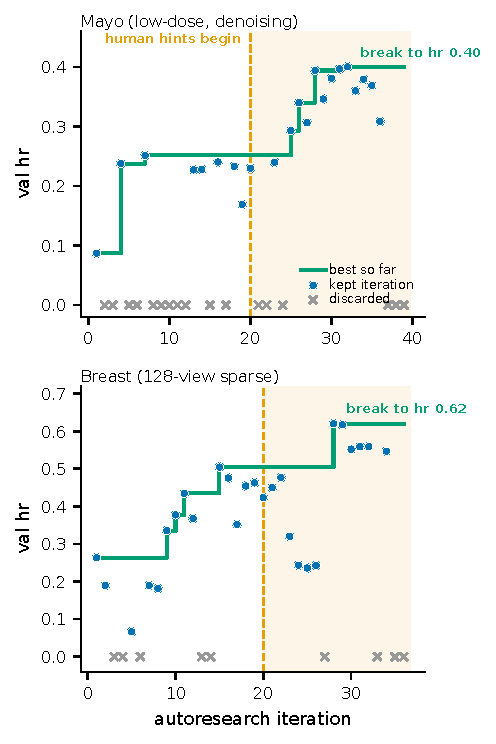
\includegraphics[width=\columnwidth]{sfig_hint_climb.pdf}}
\caption{Compact-solver search trajectories. Top: Mayo (low-dose). Bottom: breast (128-view sparse). Points are per-iteration validation headroom (discarded iterations shown at hr 0); the step line is the best value so far. On both datasets the agent's own first 20 iterations plateau (hr $\approx0.25$ Mayo, $\approx0.50$ breast); the decisive break comes only in the hinted second half (shaded) --- to hr 0.40 and 0.62 respectively.\label{fig:hintclimb}}
\end{figure}

\textbf{Mayo vs breast contrast.} On Mayo the compact optimum is an evolved field-of-experts plus multi-scale bilateral denoiser (hr 0.324 at $\sim$0.00097 M params), statistically tied with the top tier at the 1\,\% level. On a denoising problem, a tiny denoiser suffices. On sparse-view breast, that same denoiser fails; data-consistency is the differentiator.\cite{adler2018lpd} This problem-dependence is the practical face of the known-operator principle\cite{maier2019knownop,maier2022review}: embedding the exact forward operator cannot raise, and usually lowers, the maximum error bound, and it curbs the hallucination risk of unconstrained learned maps.\cite{maier2019gentle,ongie2020} The agent re-derived each optimum; it did not transfer.

\textbf{Human role in this study.} The recombination \emph{strategy} was a human idea, on both datasets. On Mayo the human repeatedly asked whether more parameter-efficient approaches existed and explicitly suggested combining the pieces. On breast the finale was framed as a cross-method recombination and steered away from copying Mayo. The agent executed and mechanistically refined; it did not originate the recombination strategy.

%============================================================
\section{Noise model and no-retrain protocol}\label{sec:s6}

The full noiseless and noisy breast boards, and the framework-axis reading of the reversal, are now in the main text; this section records only the exact noise protocol behind the re-evaluation.

Poisson photon noise per Eq.~(6) of the main text, $I_0=10^5$, applied to the 200 test sinograms with a fixed seed (deterministic; every method sees the identical noisy input). RMS of the sinogram perturbation $\approx0.012$ (line-integral units), $\sim$1.8\,\% at the thickest ray. Supervised methods load their noiseless checkpoint and skip training; per-scene/classical methods re-fit on the noisy input. The FBP baseline is recomputed from the noisy sinogram, so hr measures improvement over the noisy FBP and the comparison is fair within the noisy board.

%============================================================
\section{Agent-behavior --- extended account}\label{sec:s7}

This account follows the autoresearch paradigm of automated open-ended scientific discovery\cite{lu2024aiscientist} realized through LLM code agents that resolve real software tasks\cite{yang2024sweagent,jimenez2024swebench} and physics-informed agentic development in adjacent imaging fields.\cite{zaiss2026agent4mr}

\textbf{Strengths.} Fast paper$\to$code; strong hyper-parameter optimization; strict fixed-budget discipline; scales evaluation across many parallel benchmarks; follows well-decomposed instructions.

\textbf{Weaknesses.} Does not invent new methods. Must be forced to recombine (converges early and pads if unsupervised --- one breast sub-run replayed identical configs until an audit caught it). CT-image vision misses obvious artifacts, so numbers are the source of truth. Long tasks must be decomposed or even a 1M-token context is exhausted. Overfits to the task/metric (not only an agent trait).

\textbf{Human meta-strategies (repeatable, same on both datasets).} Persistence/breadth (keep asking for more directions); recombination (the idea to assemble pieces); redirection (do not mimic the other dataset); auditing (catch padding, enforce budget, fix provenance). The defensible claim: agent = tireless, mechanistically reasoning, self-modifying executor; human = strategist $+$ auditor.

%============================================================
\section{Additional results and the live leaderboard}\label{sec:s8}

One further figure is included here. Figure~\ref{fig:effectsize} shows, on the breast board ($n=200$), the effect size (Cohen's $d_z$) against the raw $\Delta$hr to the champion for each solver; with $n=200$ even small hr gaps are highly significant, in contrast to the low-power $n=5$ Mayo setting. The parameter/accuracy trade-off itself --- for both datasets --- is Figure~2 of the main text, and the per-step climb is quantified in the recombination-arc tables above (Tables~\ref{tab:s5mayoarc} and~\ref{tab:s5arc}).

\begin{figure}[tbp]
\centerline{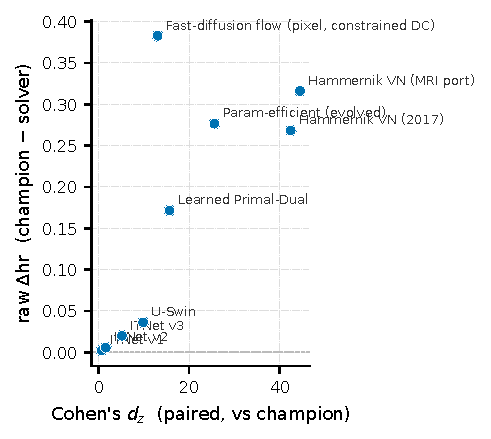
\includegraphics[width=\columnwidth]{sfig_effectsize.pdf}}
\caption{Effect size on the breast board ($n=200$): Cohen's $d_z$ versus raw $\Delta$hr against the champion, one point per solver. Large $|d_z|$ at $n=200$ is why the breast board separates cleanly, unlike the $n=5$ Mayo board.\label{fig:effectsize}}
\end{figure}

\textbf{Everything that did not fit the paper is public.} The complete results live in the repository and the live dashboard:
\begin{center}
\url{https://github.com/akmaier/Agent4CT}\\
\url{https://akmaier.github.io/Agent4CT/}
\end{center}
The dashboard hosts the full leaderboards for all datasets --- Mayo, noiseless breast, and the noisy re-evaluation --- with every solver's per-iteration trajectory. Each iteration carries an immutable provenance record: the exact configuration, the reconstruction, and the frozen metric, so any number in this paper can be traced to the run that produced it. The repository additionally holds the Mayo significance forest plot and solver$\times$metric matrix, the val-vs-test selection-honesty curves, the effort-timeline figure, the noiseless-versus-noisy reconstruction montages for the top solvers, and the per-solver design docs and \texttt{CONFIG} defaults.

% Bibliography style (WileyNJD-AMA.bst) is set by the AMA class option.
\bibliography{refs}

\end{document}
